\chapter{Implementation of CI Pipeline} \label{ci_pipeline}
\acrshort{ci}/\acrshort{cd} is all about delivering frequent, incremental changes to the application so that you can get regular feedback. But faster delivery
of the code should not affect the quality of the code. Therefore, a reliable and efficient automated testing system is required to ensure that the code is 
working as expected.

\textbf{Automated testing}/\textbf{Continuous Testing} is one of the cornerstone of \acrshort{ci}/\acrshort{cd}. It is the process of executing automated tests as part of the 
software delivery pipeline to obtain immediate feedback on the software and its quality \cite{10434454}. These scripts eliminate the need for regular manual
testing and validate the source code sequentially. By using continuous testing, developers can identify and fix bugs early in the development process, ensuring
the quality of the code. During the development of the framework, a \acrshort{ci} pipeline is implemented using GitHub Actions. This pipeline is responsible 
for running the framework on every commit to the repository. A detailed explanation of the pipeline is provided in the following sections.

\section{Version Control Strategy}
As discussed in Section \ref{version_control}, different strategies can be implemented for organizing a project. The modules present in our organization uses the 
Git Flow strategy. Here, the two long running branches, \texttt{main} and \texttt{develop} are used and feature branches are created from the \texttt{develop}
to tackle the new features. While implementing the framework, I have used the GitHub Flow strategy as it is simple and easy for a single developer. 
\newpage
\begin{figure}[!ht]
    \centering
    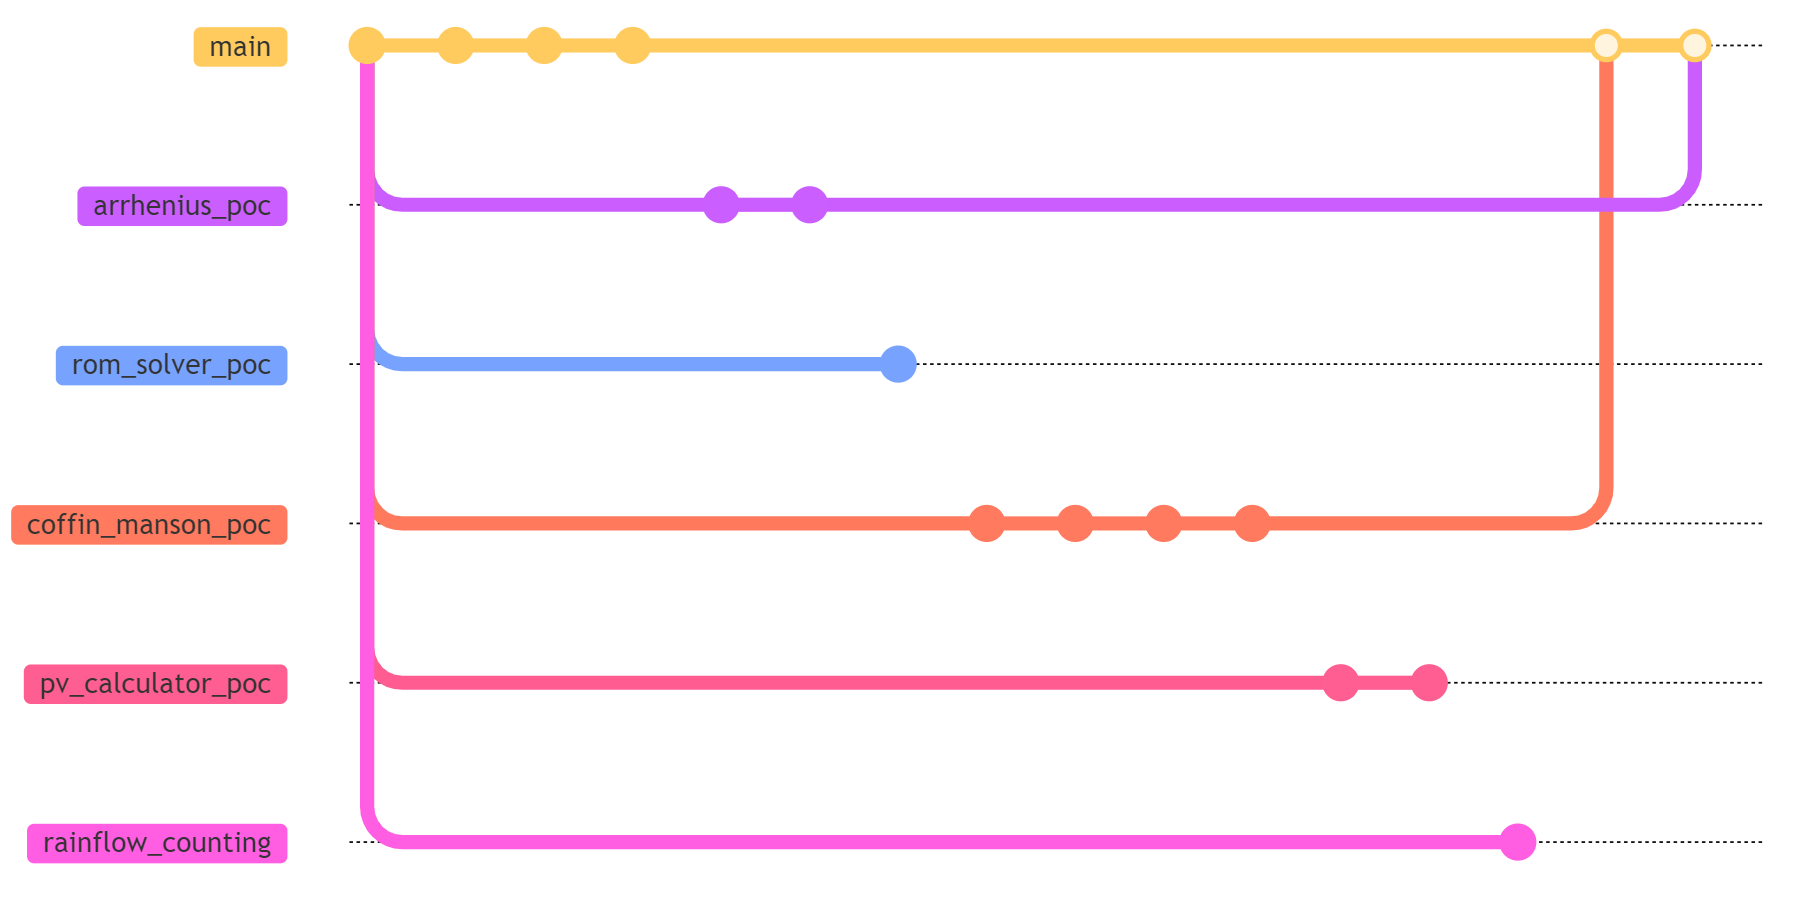
\includegraphics[width=0.9\textwidth]{Images/thesis_branching_strategy.png}
    \caption{Branching strategy for the framework}
    \label{branching_strategy}
\end{figure}

From the figure \ref{branching_strategy}, the \texttt{main} branch contains the stable code required for running the modules. Since, the framework needs to be
tested and implemented for all the modules, develop branches are created from the \texttt{main} branch. Each of the develop branch contains the code for a 
specific module. This is beneficial as the code for each module is isolated and the main source code is not affected. Once the code is tested and implemented, 
the code is merged to the \texttt{main} branch. During any commit to the develop branch, the \acrshort{ci} pipeline is triggered which builds and executes the 
module.

\section{GitHub Actions}
%# What is it?
Since the modules created by the developers and the framework are being hosted on our GitHub organization, the ideal choice for implementing the \acrshort{ci} pipeline was GitHub Actions.
GitHub Actions is a CI/CD service that makes it easy to automate tasks based on events that occur in the GitHub repository\cite{9463074}. For example, a 
trigger can be set up to run the run the pipeline based on the events like push, merge, pull request, etc. Figure \ref{github_actions_flowchart} shown below
explains the software development lifecycle and the usage of \acrshort{ci}/\acrshort{cd} in the process.\newline
\begin{figure}[!ht]
    \centering
    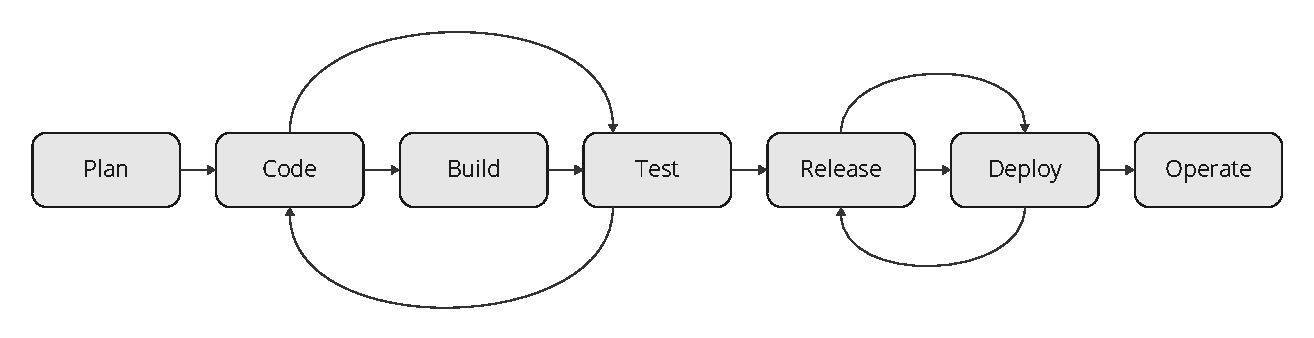
\includegraphics[width=1\textwidth]{Images/github_actions_flowchart.pdf}
    \caption{Software development lifecycle}
    \label{github_actions_flowchart}
\end{figure}

GitHub Actions is implemented after step 2 in the figure \ref{github_actions_flowchart}. After updating the codebase, the developers pushes the code to the
repository which triggers the \acrshort{ci} pipeline. This pipeline executes a script which validates the developer's code. If any exception is 
raised, the pipeline fails, preventing the code from being merged and sends a notification to the developer. Otherwise, the build is successful and the code 
is merged to the main branch.

\subsection{Components of GitHub Actions}
\subsubsection{Workflows}
This pipeline is implemented in a \texttt{.yml} or a \texttt{.yaml} file which is a superset of \acrshort{json}. This workflow file contains the configuration of 
the pipeline. This file is usually stored in the \texttt{.github/workflows} directory in the repository. 

\renewcommand{\lstlistingname}{Code}
\begin{lstlisting}[language=yaml, caption=Example of a GitHub Actions workflow file, label=workflow_file]
name: MOO Module Framework

on:
  push:
    branches:
      - arrhenius_poc

jobs:
  Run_MOO_module_framework:
    runs-on: [self-hosted, MOO_WINDOWS]

    steps:
      - name: Checkout repository
        uses: actions/checkout@v2

      - name: Set up Python
        uses: actions/setup-python@v2
        with:
          python-version: "3.12"

      - name: Install dependencies
        run: |
          python -m pip install --upgrade pip
          python install -r requirements.txt

      - name: Run main.py
        run: python main.py
\end{lstlisting}  

\subsubsection{Events}
Events are the triggers which starts the workflow. We can assign events from GitHub like push, pull to start the workflow. We can also assign the trigger to a 
specific branch or tag. In code snippet \ref{workflow_file}, the workflow is setup to trigger on every push to the \texttt{arrhenius\_poc} branch. 

\subsubsection{Jobs}
Jobs are a set of defined tasks which are executed when the pipeline is triggered. Each job is assigned to a runner which is a virtual machine that runs the 
job. Jobs contains a set of steps which are executed sequentially. If any step fails, the job is marked as failed and the pipeline comes to a halt. In code snippet 
\ref{workflow_file}, the job \texttt{Run\_MOO\_module\_framework} is assigned to a self-hosted runner with the label \texttt{MOO\_WINDOWS}. This 
job contains 4 steps which are executed sequentially.

\subsubsection{Actions}
Actions is a GitHub Actions feature that contains specific custom program performing a task. These actions are reusable and can be used in multiple workflows.
It helps in reducing the number of lines of code in the workflow file. From the code \ref{workflow_file}, the actions \texttt{actions/checkout@v2} and 
\texttt{actions/setup-python@v2} are used to checkout the repository and setup the python environment respectively in the runner. There are several actions 
available in the GitHub marketplace which can be used in the workflow.

\subsubsection{Runners}
Runners are servers which assist in the running the workflow. GitHub provides Ubuntu Linux, Microsoft Windows and Ubuntu runners which are hosted by GitHub.
Apart from these, we can host our own runners which can be used to run the workflow. In our organization, the workflow is usually ran in one of our lab computers
which is setup as a self-hosted runner. To identify the runner, a label is assigned to the runner, so that the workflow can be run in a desired runner. 
In the example shown in Code \ref{workflow_file}, the job is assigned to a self-hosted runner with the label \texttt{MOO\_WINDOWS}. 

The disadvantage of runners in GitHub Actions is that the runners can only run one job at a time. Additionally, needs to be online all the time to execute the 
workflow. 

\section{Summary}
The implementation of the \acrshort{ci} pipeline is a crucial step in testing the integration capabilities of modules using the framework. The pipeline is set to trigger on every push to
a specific branch. On triggering, the pipeline gets the files from the repository, sets up the python environment, installs the dependencies and runs the 
\texttt{main.py}, which calls the framework. If any exception is raised during steps, the pipeline fails and sends a notification to the developer. Otherwise,
the pipeline is marked as successful and the code is merged to the branch.